\documentclass[]{article}
\usepackage{lmodern}
\usepackage{amssymb,amsmath}
\usepackage{ifxetex,ifluatex}
\usepackage{fixltx2e} % provides \textsubscript
\ifnum 0\ifxetex 1\fi\ifluatex 1\fi=0 % if pdftex
  \usepackage[T1]{fontenc}
  \usepackage[utf8]{inputenc}
\else % if luatex or xelatex
  \ifxetex
    \usepackage{mathspec}
  \else
    \usepackage{fontspec}
  \fi
  \defaultfontfeatures{Ligatures=TeX,Scale=MatchLowercase}
\fi
% use upquote if available, for straight quotes in verbatim environments
\IfFileExists{upquote.sty}{\usepackage{upquote}}{}
% use microtype if available
\IfFileExists{microtype.sty}{%
\usepackage{microtype}
\UseMicrotypeSet[protrusion]{basicmath} % disable protrusion for tt fonts
}{}
\usepackage[margin=1in]{geometry}
\usepackage{hyperref}
\hypersetup{unicode=true,
            pdftitle={A Brief Introduction to Bandwidth Selection Methods for Univariate Kernel Density Estimation},
            pdfauthor={Brad Stieber},
            pdfborder={0 0 0},
            breaklinks=true}
\urlstyle{same}  % don't use monospace font for urls
\usepackage{color}
\usepackage{fancyvrb}
\newcommand{\VerbBar}{|}
\newcommand{\VERB}{\Verb[commandchars=\\\{\}]}
\DefineVerbatimEnvironment{Highlighting}{Verbatim}{commandchars=\\\{\}}
% Add ',fontsize=\small' for more characters per line
\usepackage{framed}
\definecolor{shadecolor}{RGB}{248,248,248}
\newenvironment{Shaded}{\begin{snugshade}}{\end{snugshade}}
\newcommand{\KeywordTok}[1]{\textcolor[rgb]{0.13,0.29,0.53}{\textbf{{#1}}}}
\newcommand{\DataTypeTok}[1]{\textcolor[rgb]{0.13,0.29,0.53}{{#1}}}
\newcommand{\DecValTok}[1]{\textcolor[rgb]{0.00,0.00,0.81}{{#1}}}
\newcommand{\BaseNTok}[1]{\textcolor[rgb]{0.00,0.00,0.81}{{#1}}}
\newcommand{\FloatTok}[1]{\textcolor[rgb]{0.00,0.00,0.81}{{#1}}}
\newcommand{\ConstantTok}[1]{\textcolor[rgb]{0.00,0.00,0.00}{{#1}}}
\newcommand{\CharTok}[1]{\textcolor[rgb]{0.31,0.60,0.02}{{#1}}}
\newcommand{\SpecialCharTok}[1]{\textcolor[rgb]{0.00,0.00,0.00}{{#1}}}
\newcommand{\StringTok}[1]{\textcolor[rgb]{0.31,0.60,0.02}{{#1}}}
\newcommand{\VerbatimStringTok}[1]{\textcolor[rgb]{0.31,0.60,0.02}{{#1}}}
\newcommand{\SpecialStringTok}[1]{\textcolor[rgb]{0.31,0.60,0.02}{{#1}}}
\newcommand{\ImportTok}[1]{{#1}}
\newcommand{\CommentTok}[1]{\textcolor[rgb]{0.56,0.35,0.01}{\textit{{#1}}}}
\newcommand{\DocumentationTok}[1]{\textcolor[rgb]{0.56,0.35,0.01}{\textbf{\textit{{#1}}}}}
\newcommand{\AnnotationTok}[1]{\textcolor[rgb]{0.56,0.35,0.01}{\textbf{\textit{{#1}}}}}
\newcommand{\CommentVarTok}[1]{\textcolor[rgb]{0.56,0.35,0.01}{\textbf{\textit{{#1}}}}}
\newcommand{\OtherTok}[1]{\textcolor[rgb]{0.56,0.35,0.01}{{#1}}}
\newcommand{\FunctionTok}[1]{\textcolor[rgb]{0.00,0.00,0.00}{{#1}}}
\newcommand{\VariableTok}[1]{\textcolor[rgb]{0.00,0.00,0.00}{{#1}}}
\newcommand{\ControlFlowTok}[1]{\textcolor[rgb]{0.13,0.29,0.53}{\textbf{{#1}}}}
\newcommand{\OperatorTok}[1]{\textcolor[rgb]{0.81,0.36,0.00}{\textbf{{#1}}}}
\newcommand{\BuiltInTok}[1]{{#1}}
\newcommand{\ExtensionTok}[1]{{#1}}
\newcommand{\PreprocessorTok}[1]{\textcolor[rgb]{0.56,0.35,0.01}{\textit{{#1}}}}
\newcommand{\AttributeTok}[1]{\textcolor[rgb]{0.77,0.63,0.00}{{#1}}}
\newcommand{\RegionMarkerTok}[1]{{#1}}
\newcommand{\InformationTok}[1]{\textcolor[rgb]{0.56,0.35,0.01}{\textbf{\textit{{#1}}}}}
\newcommand{\WarningTok}[1]{\textcolor[rgb]{0.56,0.35,0.01}{\textbf{\textit{{#1}}}}}
\newcommand{\AlertTok}[1]{\textcolor[rgb]{0.94,0.16,0.16}{{#1}}}
\newcommand{\ErrorTok}[1]{\textcolor[rgb]{0.64,0.00,0.00}{\textbf{{#1}}}}
\newcommand{\NormalTok}[1]{{#1}}
\usepackage{graphicx,grffile}
\makeatletter
\def\maxwidth{\ifdim\Gin@nat@width>\linewidth\linewidth\else\Gin@nat@width\fi}
\def\maxheight{\ifdim\Gin@nat@height>\textheight\textheight\else\Gin@nat@height\fi}
\makeatother
% Scale images if necessary, so that they will not overflow the page
% margins by default, and it is still possible to overwrite the defaults
% using explicit options in \includegraphics[width, height, ...]{}
\setkeys{Gin}{width=\maxwidth,height=\maxheight,keepaspectratio}
\IfFileExists{parskip.sty}{%
\usepackage{parskip}
}{% else
\setlength{\parindent}{0pt}
\setlength{\parskip}{6pt plus 2pt minus 1pt}
}
\setlength{\emergencystretch}{3em}  % prevent overfull lines
\providecommand{\tightlist}{%
  \setlength{\itemsep}{0pt}\setlength{\parskip}{0pt}}
\setcounter{secnumdepth}{0}
% Redefines (sub)paragraphs to behave more like sections
\ifx\paragraph\undefined\else
\let\oldparagraph\paragraph
\renewcommand{\paragraph}[1]{\oldparagraph{#1}\mbox{}}
\fi
\ifx\subparagraph\undefined\else
\let\oldsubparagraph\subparagraph
\renewcommand{\subparagraph}[1]{\oldsubparagraph{#1}\mbox{}}
\fi

%%% Use protect on footnotes to avoid problems with footnotes in titles
\let\rmarkdownfootnote\footnote%
\def\footnote{\protect\rmarkdownfootnote}

%%% Change title format to be more compact
\usepackage{titling}

% Create subtitle command for use in maketitle
\newcommand{\subtitle}[1]{
  \posttitle{
    \begin{center}\large#1\end{center}
    }
}

\setlength{\droptitle}{-2em}
  \title{A Brief Introduction to Bandwidth Selection Methods for Univariate
Kernel Density Estimation}
  \pretitle{\vspace{\droptitle}\centering\huge}
  \posttitle{\par}
  \author{Brad Stieber}
  \preauthor{\centering\large\emph}
  \postauthor{\par}
  \date{}
  \predate{}\postdate{}


\begin{document}
\maketitle
\begin{abstract}
Univariate kernel density estimation allows an analyst to get a quick
glimpse of the distributional properties for some data vector they have
in hand. Of utmost importance in kernel density estimation is selecting
the bandwidth, which controls the smoothness of the estimate.
Insufficient smoothing leads to an estimate which may detect spurious
modality, and over-smoothing may obscure important patterns within the
data. In this report, we discuss various methods for selecting an
optimal bandwidth for univariate kernel density estimation. We discuss
Silverman's rule of thumb (1986), a cross-validation technique, Sheather
and Jones' plug-in estimator (1991), and Terrell's maximal smoothing
principle (1990). We visualize results from univariate density
estimation using the different bandwidths for various data vectors,
referencing a function written in the \texttt{R} computing environment.
We also developed and deployed a
\href{http://www.statlab.wisc.edu/shiny/Bandwidths_For_UnivariateKDE/}{Shiny-based
web application} which provides an interactive summary of some of the
important aspects of this report.
\end{abstract}

\section{Introduction}\label{introduction}

Kernel density estimation (KDE) allows a data analyst to estimate the
probability density \(f\) of some univariate data vector they have. An
analyst may use KDE for a quick visualization, or even implement the
results from their KDE into a simulation study. The results of a KDE are
typically visualized as curves, which may provide a more refined view of
the modality within a data vector than a histogram.\footnote{The
  refinement of the display may come at the cost of overemphasizing the
  smoothness of the estimator. It is good practice to overlay a
  histogram plot with the KDE.}

A kernel density estimate requires the selection of a kernel (\(K\)),
and a bandwidth (\(h\)). In this report, our focus is on selecting the
bandwidth \(h\). The bandwidth controls how smooth our estimate of the
underlying density is. If we select a large bandwidth, we will smooth
out some of the interesting features of the distribution of the data. If
we select a small bandwidth, our density estimate may be too ``wiggly'',
and over-exaggerate random perturbations in the data as multi-modality.
While many methods exist for selecting a bandwidth, it should be noted
that no universally best method has been found (Givens and Hoeting 2013,
332).

Suppose we have a sample \(x_1, x_2, \ldots, x_n\) which are i.i.d.
observations from some density \(f\). We wish to estimate \(f\) using
\(\hat{f}\) for an analysis. We can use the kernel density estimator
\(\hat{f}\) to approximate the density.

The kernel density estimate of \(f\) at \(x\) is:

\[\widehat{f_h}(x) = \frac{1}{nh} \sum_{i = 1}^{n}K\left(\frac{x - x_i}{h}\right) \]

where \(h\) is the smoothing parameter known as the bandwidth, and \(K\)
is a kernel function which satisfies \(\int{K(x)dx} = 1\). In general,
\(K\) should also satisfy the conditions (Sheather 2004)

\[\int{yK(y)dy} = 0\] \[\int{y^2K(y)dy} = \mu_2(K) > 0.\]

The kernel function is generally chosen to be a unimodal probability
density function that is symmetric around zero. Popular choices include
the Gaussian kernel (\(K(x) = \phi(x)\)), the Epanechnikov kernel
(\(K(x) = \frac{3}{4}(1-x^2)*\mathbb{I}(\left|x \right| <1)\)), and the
triangular kernel
(\(K(x) = (1 - \left|x\right|)*\mathbb{I}(\left|x\right| < 1)\)).
Provided the kernel function \(K(x)\) satisfies the aforementioned
conditions, the choice of kernel will not be as important the selection
of a bandwidth.

\begin{figure}[htbp]
\centering
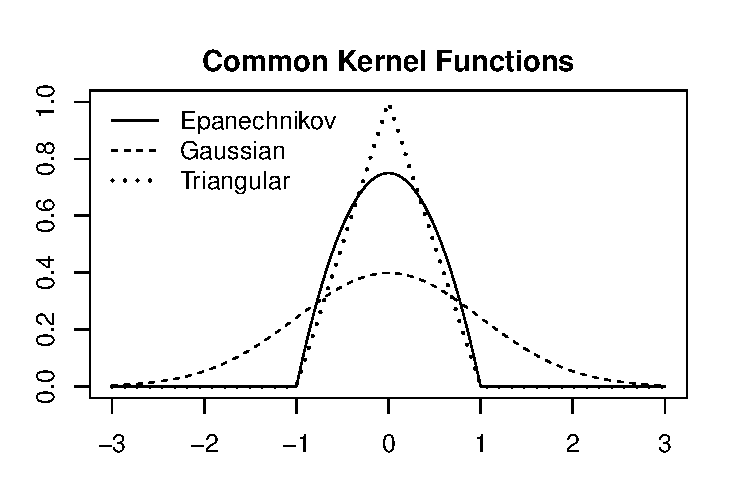
\includegraphics{FinalReport_files/figure-latex/unnamed-chunk-2-1.pdf}
\caption{Three Common Kernel Functions: the solid line is the
Epanechnikov kernel, the dashed line is the standard Gaussian kernel,
and the dotted line is the Triangular kernel}
\end{figure}

We use the bandwidth to control how much weight we apply to observations
around the \(x\) for which we are evaluating \(\widehat{f_h}(x)\). If
\(h\) is too small, we assign density too locally, resulting in wiggly
estimates; however, if we select \(h\) to be too large, we spread
density too diffusely, smoothing out interesting features of the data
(Givens and Hoeting 2013). We have illustrated the effect of bandwidth
in Figure 2, where we have evaluated \(\widehat{f_h}(x)\) for 200 points
from the \(N(2, 3)\) density.

\begin{figure}[htbp]
\centering
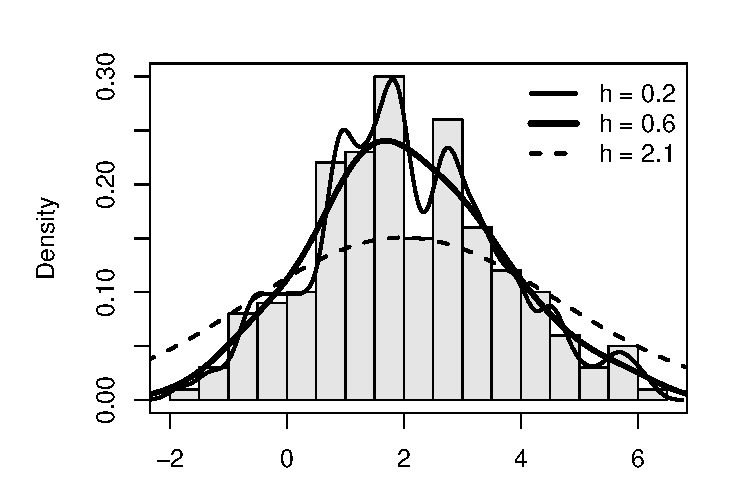
\includegraphics{FinalReport_files/figure-latex/unnamed-chunk-3-1.pdf}
\caption{Kernel density estimates using 3 bandwidths for 500 points from
N(2, 3)}
\end{figure}

We have provided three density estimates in Figure 2, each using a
Gaussian kernel, but different bandwidths. The lighter solid line is too
small of a bandwidth (\(h\) = 0.2), as it is too sensitive to local
perturbations. The dashed line is too large of a bandwidth (\(h\) = 2),
so it over-smooths the interesting components of the distribution. The
heavy line (\(h\) = 0.6) seems to be a fairly respectable bandwidth; it
does not over-smooth the data, and it also highlights some of the
interesting features of the data.

\newpage

\section{Methods for evaluating KDE}\label{methods-for-evaluating-kde}

To calculate \(\widehat{f_h}(x)\), we need to compute an estimate for
every observation \(x_i\), based on the \(n-1\) remaining observations
in the data. This computation requires \(n (n-1)\) computations to
calculate the final estimate. To get around such a computationally
intensive calculation, techniques such as linear binning and Fast
Fourier Transforms are used (both are implemented in \texttt{R}'s
\texttt{density} function).

Computing the kernel density estimator amounts to piling up mass around
each \(x\), then summing the mass up over \(x_1, x_2, \ldots, x_n\).
Figure 3 demonstrates this computation. We start with 10 i.i.d.
observations from \(N(0,1)\), which are the red triangles in the plot.
Using a Gaussian kernel, we compute the densities (scaled by \(1/nh\))
for each \(x\), which are the solid blue curves in the plot. We then sum
across these pointwise densities and are left with our final KDE, which
is the thick black curve. We have provided plots for a large bandwidth
and a small bandwidth, demonstrating the micro and macro effects of
bandwidth selection.

\begin{figure}

{\centering 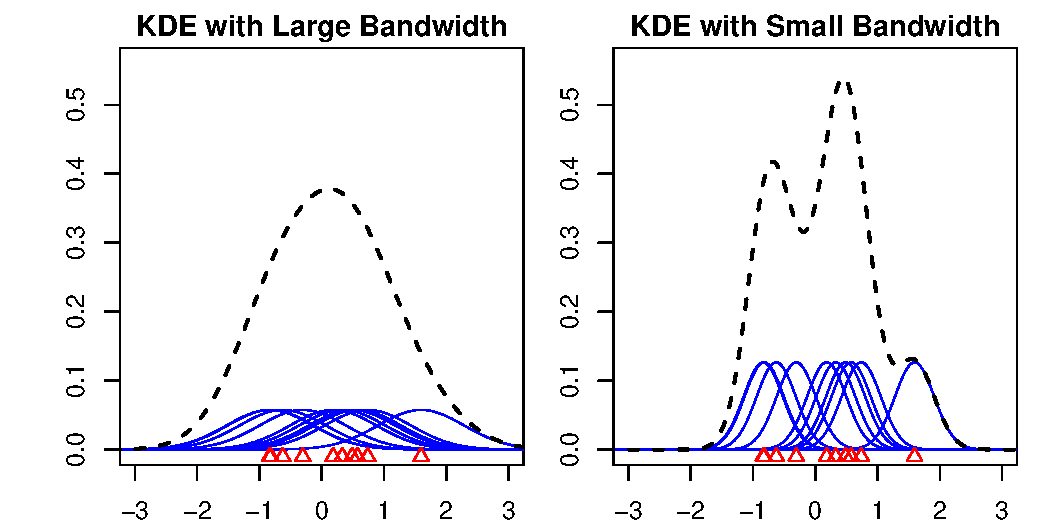
\includegraphics{FinalReport_files/figure-latex/unnamed-chunk-4-1} 

}

\caption{Demonstration of KDE computation. Red triangles are 10 i.i.d. data points from N(0,1). The solid blue lines are scaled densities at each data point. The thick black line is the final KDE. Left panel uses a large bandwidth (more smoothing), right panel uses a small bandwidth (less smoothing).}\label{fig:unnamed-chunk-4}
\end{figure}

\subsection{Evaluating $\widehat{f}_h(x)$ as an Estimator}

Along with the computation of \(\widehat{f_h}(x)\), it is also important
to assess the quality of \(\hat{f}\) as an estimator of \(f\). One
choice would the be the Integrated Squared Error (ISE):

\[ISE(h) = \int_{-\infty}^{\infty} \left(\hat{f}(x) - f(x)\right)^2dx.\]
ISE calculates the squared error for \emph{this} sample. It might be
reasonable to average ISE over \emph{all} samples, resulting in Mean
Integrated Squared Error (MISE): \(MISE(h) = E\left(ISE(h)\right).\)

We can rewrite \(MISE(h)\) as:

\[MISE(h) = \int_{-\infty}^{\infty}MSE_h\left(\hat{f}(x)\right)dx,\] and
decompose \(MSE\) as \(MSE = bias^2 + var\):

\[MISE(h) = \int_{-\infty}^{\infty} var\left(\widehat{f_h}(x)\right) + bias\left(\widehat{f_h}(x)\right)^2 dx.\]
Givens and Hoeting (2013, 327) say of the distinction between \(ISE\)
and \(MISE\)\footnote{The reader may be interested in our focus on
  squared error, instead of opting for the \(L_1\) norm. While the
  \(L_1\) norm is theoretically appealing, due to its invariance under
  one-to-one smooth transformations, it can be somewhat difficult to
  analyze mathematically. For this reason it is neglected here.}:

\begin{quote}
The distinction is essentially one between the statistical concepts of
loss and risk. Using ISE(h) is conceptually appealing because it
assesses the estimator's performance with the observed data. However,
focusing on MISE(h) is an effective way to approximate ISE-based
evaluation while reflecting the sensible goal of seeking optimal
perfomance on average over many data sets.
\end{quote}

Givens and Hoeting (2013, 331) derived \(E[\widehat{f_h}(x)]\) as:

\[E[\widehat{f_h}(x)] = f(x) + \frac{1}{2} h^2 \sigma_K^2f^{''}(x) + o(h^2),\]

where \(\sigma_K^2\) is the variance of \(K\) (\(\int z^2 K(z) dz\)). So
that
\(\left(bias(\widehat{f_h}(x))\right)^2 = \frac{1}{4} h^4\sigma_K^4 (f^{''})^2 + o(h^4)\),
and integrating \(bias^2\) results in:

\[\int bias\left(\hat{f}(x)\right)^2 dx = \frac{1}{4} h^4 \sigma_K^4 R(f^{''}) + o(h^4),\]

where \(R\) is a measure of the roughness of a function g:

\[R(g) = \int_{-\infty}^{\infty}g^2(z) dz.\]

It can also be shown that
\(var\left(\hat{f}(x)\right) = \frac{1}{nh}f(x)R(K) + o(\frac{1}{nh})\),
and integrating \(var\) results in:

\[\int var\left(\hat{f}(x)\right)dx = \frac{R(K)}{nh} + o\left(\frac{1}{nh}\right).\]

Adding \(bias^2\) and \(var\) together results in:

\[
\begin{aligned}
MISE(h) &= \frac{R(K)}{nh} + o\left(\frac{1}{nh}\right) + \frac{1}{4}h^4 \sigma_K^4R(f^{''}) + o\left(h^4\right) \\
&= AMISE(h) + o\left(\frac{1}{nh} + h^4\right),
\end{aligned}
\] where \(AMISE\) is the Asymptotic Mean Integrated Squared Error. If
\(nh \rightarrow \infty\) and \(h \rightarrow 0\) as
\(n \rightarrow \infty\), then \(MISE(h) \rightarrow 0\).

Inspection of the \(bias^2\) and \(var\) components of \(MISE(h)\) with
respect to the bandwidth \(h\) provides an example of the bias-variance
tradeoff. Selecting a small value of \(h\) increases variance by
producing a wiggly estimate, but reduces bias. Selecting a large value
of \(h\) reduces the variance of the estimator, but increases the bias
due to over-smoothing. To find an optimal value, we must balance the
bias and variance components of \(MISE\), a typical theme in statistics.

Finding an optimal bandwidth \(h_{AMISE}\), is straightforward:

\[
\begin{aligned}
AMISE &= \frac{R(K)}{nh} + \frac{h^4\sigma_K^4R(f^{''})}{4}\\
\frac{dAMISE}{dh} &= \frac{-R(K)}{nh^2} + h^3\sigma_K^4 R(f^{''})\\
0 &= \frac{-R(K)}{n} + h^5 \sigma_K^4 R(f^{''}) \\
h^5 &= \frac{R(K)}{n\sigma_K^4 R(f^{''})} \\
h_{AMISE} &= \left(\frac{R(K)}{n\sigma_K^4R(f^{''})}\right)^{\frac{1}{5}}.
\end{aligned}
\]

All of the components of \(h_{AMISE}\) are known to us, except for
\(R(f^{''})\). \(R(f^{''})\) possesses a key to determining an
appropriate bandwidth. Of \(R(f^{''})\), Sheather (2004, 589) states:

\begin{quote}
Thus, the functional \(R(f^{''})\) is a measure of the underlying
roughness or curvature. In particular, the larger the value of
\(R(f^{''})\) is, the larger is the value of AMISE (i.e., the more
difficult it is to estimate \(f\)) and the smaller is the value of
\(h_{AMISE}\) (i.e., the smaller the bandwidth needed to capture the
curvature in \(f\)).
\end{quote}

\section{Bandwidth Selection}\label{bandwidth-selection}

The possible choices for bandwidth depend on navigating around the fact
that \(R(f^{''})\) is unknown. We investigate four bandwidth selection
strategies which employ different methods to circumvent not knowing
\(R(f^{''})\).

\begin{itemize}
\item
  Cross validation: choose a different objective function based on
  \(ISE\), and use a leave one out (LOO) cross validation estimator to
  find \(\int \hat{f}_h f\)
\item
  Silverman's ROT: replace \(f\) with the \(N(0, \sigma^2)\) density
\item
  Sheather-Jones: empirically estimate \(f''(x)\) to find \(h\) in a
  two-step method
\item
  Terrell's Maximal Smoothing: minimize \(R(f^{''})\) for a given
  \(\sigma\)
\end{itemize}

\subsection{Unbiased Cross Validation}\label{unbiased-cross-validation}

We can represent integrated squared error as:

\[
ISE(h) = \int \left(\hat{f}_h - f\right) = \int\hat{f}_h^2 - 2\int \hat{f}_hf + \int f^2.
\]

In \(ISE(h)\), only the first two terms rely on \(h\), and the first
term is entirely known. We can estimate the second term
(\(2\int \hat{f}_hf = 2 E(\hat{f}_h)\)) using
\(2/n \sum_{i=1}^{n}\hat{f}_{-i}(x_i)\). Where

\[
\hat{f}_{-i}(x_i) = \frac{1}{h(n-1)}\sum_{j \neq i} K\left(\frac{x_i - x_j}{h}\right)
\]

is the leave-one-out kernel density estimator at \(x_i\) using all of
the data except \(x_i\).

We then attempt to minimize

\[
UCV(h) = R(\hat{f}) - \frac{2}{n} \sum_{i = 1}^{n} \hat{f}_{-i}(x_i
\] with respect to \(h\).

\(UCV(h)\) is called the ``unbiased cross-validation'' criterion because
\(E\left[UCV(h) + R(f)\right] = MISE(h)\) (Givens and Hoeting 2013,
333). To estimate the unbiased cross validation bandwidth for a data
vector \texttt{x} in \texttt{R}, a user can write \texttt{bw.ucv(x)}.
Along with ``unbiased cross-validation'', it is sometimes referred to as
``least-squares cross validation'' as it minimizes the integrated
squared error. When we refer to the cross-validated bandwidth selector,
we denote the bandwidth as \(h_{LSCV}\).

For this report, we have focused on the Gaussian kernel. \(UCV(h)\) has
a straightforward expression when a Gaussian kernel is used (equation
10.23, Givens and Hoeting (2013, 333)), which makes the computation of
\(h_{LSCV}\) rather tidy.

The unbiasedness of the objective function is a nice feature, but it
comes at the cost of imbuing \(h_{LSCV}\) with excessive variance
(Jones, Marron, and Sheather 1992, 6). The objective function \(UCV\)
tends to depend too heavily on the sample in hand, since it is still
random (unlike \(MISE\), which is averaged over \emph{all} samples). The
heavy dependence on the data in hand often leads to high variation in
\(\hat{f}_h\). This excessive variation is displayed in the
\emph{Examples} section of this report.

\subsection{Silverman's Rule of Thumb}\label{silvermans-rule-of-thumb}

A simpler method relies on selecting an appropriate density to
approximate \(R(f^{''})\) in

\[
h_{AMISE} = \left(\frac{R(K)}{n\sigma_K^4R(f^{''})}\right)^{\frac{1}{5}}.
\]

If we choose \(f\) to be the normal density with mean 0 and variance
\(\sigma^2\), and use the Gaussian kernel for \(K\), we can express
\(h_{AMISE}\) as:

\[
\begin{aligned}
h_{AMISE} &= \left(\frac{(2\sqrt{\pi})^{-1}}{\frac{3}{8}\pi^{-\frac{1}{2}}\sigma^{-5}}\right)^{1/5} n^{-1/5} \\
&= 1.06\sigma n^{-\frac{1}{5}}.
\end{aligned}
\]

A natural estimate of \(\sigma\) is \(\hat{\sigma}\), the sample
standard deviation. If the true \(f\) deviates from the features of a
normal distribution (for instance, it is multimodal), this approximation
may do a poor job (i.e.~it will oversmooth). A possibility is to use the
interquartile range, which is a more robust measure of spread. We then
replace \(\hat{\sigma}\) with
\(\tilde{\sigma} = min\left[\hat{\sigma}, \frac{IQR(x)}{1.34}\right]\).
This leads to Silverman's rule of thumb:

\[
h_{SROT_1} = 1.06 \tilde{\sigma} n ^ {-\frac{1}{5}}.
\]

In our report, we replace 1.06 in the previous equation with 0.9, so
that \(h_{SROT} = \frac{0.9}{1.06} h_{SROT_1}\). This replacement
dampens some of the over-smoothing that takes place when this method is
used, and attempts to avoid missing bimodality in the distribution
(Silverman 1986, 48). In \texttt{R}, a user can obtain \(h_{SROT_1}\)
for a data vector \texttt{x} by using \texttt{bw.nrd(x)}, and can obtain
\(h_{SROT}\) by using \texttt{bw.nrd0(x)}.

The computation of \(h_{SROT}\) is fairly simple, and requires no
optimization or cross-validation scheme. The simplicity comes at a cost;
however, as this bandwidth tends to oversmooth the estimate, even after
the IQR correction is made. The over-smoothing typically gets worse as
\(f\) deviates from normality.

\subsection{Sheather-Jones Bandwidth}\label{sheather-jones-bandwidth}

Silverman's rule of thumb relies on selecting a candidate density to
estimate \(R(f^{''})\). Sheather and Jones (1991) opt for a different
approach: empirically estimate \(R(f^{''})\). An empirical estimate of
\(f^{''}\) is formulated as:

\[
\begin{aligned}
\hat{f}''(x) &= \frac{d^2}{dx^2} \left\{\frac{1}{nh_0} \sum_{i=1}^{n} L\left(\frac{x - x_i}{h_0}  \right) \right\}\\
&= \frac{1}{nh_0^3} \sum_{i=1}^{n} L''\left(\frac{x-x_i}{h_0} \right).
\end{aligned}
\]

Where \(h_0\) is another bandwidth, different from \(h\) (and typically
\(h_0 > h\) Givens and Hoeting (2013, 336)), and \(L\) is a kernel
function.

To compute the optimal bandwidth \(h_{SJ}\), Sheather and Jones use a
two-step process. First, a simple rule of thumb is used to calculate
\(h_0\). Then \(h_0\) is used to estimate \(R(f^{''})\), which is the
only unknown quantity in the expression for \(h_{AMISE}\). After
plugging in the estimator for \(R(f^{''})\) in the expression for
\(h_{AMISE}\), we arrive at the Sheather-Jones bandwidth. An expression
for the optimal bandwidth when \(L = \phi\) is in the Appendix. This
expression requires a root-finding scheme such as Newton's method. In
\texttt{R}, a user can obtain \(h_{SJ}\) for a data vector \texttt{x} by
writing \texttt{bw.SJ(x)}.

In simulation studies (summarized in Jones, Marron, and Sheather
(1996)), it was seen that \(h_{SJ}\) tended to be superior to both
\(h_{LSCV}\) and \(h_{SROT}\). In general, \(h_{SJ}\) demonstrates less
variation than \(h_{LSCV}\) and is centered near \(h_{AMISE}\) for
easy-to-estimate densities. For more difficult densities, \(h_{SJ}\)
will overshoot \(h_{AMISE}\), but is still much smaller than
\(h_{SROT}\). \(h_{SJ}\), then, seems to be a suitable compromise
between the low-variance high-bias \(h_{SROT}\) and the high-variance
low-bias \(h_{LSCV}\).

\subsection{Terrell's Maximal Smoothing
Principle}\label{terrells-maximal-smoothing-principle}

Terrell (1990) opted for a different approach in determining an optimal
bandwidth. Rather than focusing on finding a good estimator of \(f''\)
or \(R(f'')\) in the expression for \(h_{AMISE}\), Terrell chose to find
some density function \(g\) that would minimize
\(R(g'') = \int (g '' (x))^2 dx\) for a given variance \(\sigma^2\). By
minimizing \(\int (g'')^2\), we could determine an upper bound for
\(h_{AMISE}\), by using \(g\) in place of \(f\). Terrell (1990, 472)
justifies using the maximally smoothed bandwidth, because it avoids the
tendency of the under-smoothed density estimate to ``display features
such as asymmetries and multiple modes that could have come about by
chance''.

Terrell's estimate is built on the result that the
\(beta(k + 2, k + 2)\) family minimizes \(\int (f^{(k)})^2\) for a given
standard deviation (Terrell 1990, 471). For a kernel with variance 1
(e.g.~the Gaussian kernel), the maximal smoothing bandwidth is:

\[
h_{MS} =  3 \hat \sigma \left(\frac{R(K)}{35 n} \right)^{\frac{1}{5}}.
\]

The maximal smoothing principle has an intuitive justification, and its
ideas permeate through wider areas of statistical inference. It would be
desirable for an inferential scheme to prevent an analyst from claiming
features of a data set exist that may have arisen by pure chance alone
(Terrell 1990, 472). The maximal smoothing principle applies this idea
to the display of kernel density estimates.

In terms of kernel density estimation; however, the maximal smoothing
principle provides only an upper bound on the optimal bandwidth.
Silverman's rule of thumb is an over-smoother, and Terrell's maximal
smoothing bandwidth smooths out even more features of the data than
\(h_{SROT}\) does (Jones, Marron, and Sheather 1992, 9).

\section{\texorpdfstring{Examples Using the \texttt{kde}
Function}{Examples Using the kde Function}}\label{examples-using-the-kde-function}

To examine the four bandwidth selection methods we have investigated, we
use four different data vectors to investigate the changes in density
estimation as the data deviates from the normal distribution. Three
vectors are simulated, and one vector is from a real data set.\footnote{The
  \texttt{R} code used to generate the data can be found on the author's
  Github:
  \url{https://github.com/bgstieber/Project771/blob/master/Project\%20Files/DataGeneration.R}}
Our main interest is on if the bandwidth options lead to under-smoothing
or over-smoothing of the data.

We plot histograms and density estimates for each of the data vectors
using the \texttt{kde} function. The \texttt{kde} function takes in a
data vector, and calculates \(h_{SROT}\), \(h_{SJ}\), \(h_{LSCV}\), and
\(h_{MS}\). It then calculates \(\widehat{f}_h(x)\). For small data
vectors (\(n \leq 1,000\)), \texttt{kde} will calculate the densities
``by hand'', using a grid of size 512. For larger data vectors, the
function will use the \texttt{density} function in base \texttt{R}. In
addition to creating plots, the \texttt{kde} function will print the
four bandwidths, and can also return \(\widehat{f}_h(x)\) for an evenly
spaced grid of length 512 for each \(h\).

In each example, we choose a data vector and display the output from
\texttt{kde}. We then attempt to interpret the results, taking special
care to analyze the effect of each bandwidth choice on \(\hat{f}_h\).
Inspecting a kernel density estimate is not an objective task, as one
analyst may perceive different features than another. It is important to
present multiple density estimates, and iterate through different
bandwidths to arrive at a more common conclusion.

We include each \(\hat f_h\) on the same graph rather than allowing each
\(\hat f_h\) to have its own panel. This strategy allows for the other
three \(\hat f_h\)'s to act as ``reality checks'' for the \(\hat f_h\)
of the \(h\) we are focusing on. Keeping the estimates on the same graph
should allow for effective comparisons between the \(\hat f_h\)'s.

\subsection{Shiny Web Application}

In addition to the \texttt{kde} function, a Shiny-based web application
was developed and deployed
\textbf{\href{http://www.statlab.wisc.edu/shiny/Bandwidths_For_UnivariateKDE/}{here}}.
The application creates density plots for a variety of data choices, and
allows the user to investigate different bandwidths for simulated and
real-world data sets. The application also allows a user to visualize
pointwise confidence intervals for kernel density estimates using the
approximate variance (Jann (2007)), and a nonparametric bootstrap
percentile method. Additionally, the app allows a user to upload a one
column \texttt{.csv} file and investigate the kernel density estimate as
well. Screenshots of the application are in the \emph{Appendix}.

\subsection{Example 1: 300 samples from $N(2, 2^2)$}

\begin{verbatim}
##           LS CV            T MS           SJ BW Silverman's ROT 
##           0.648           0.691           0.598           0.519
\end{verbatim}

\begin{center}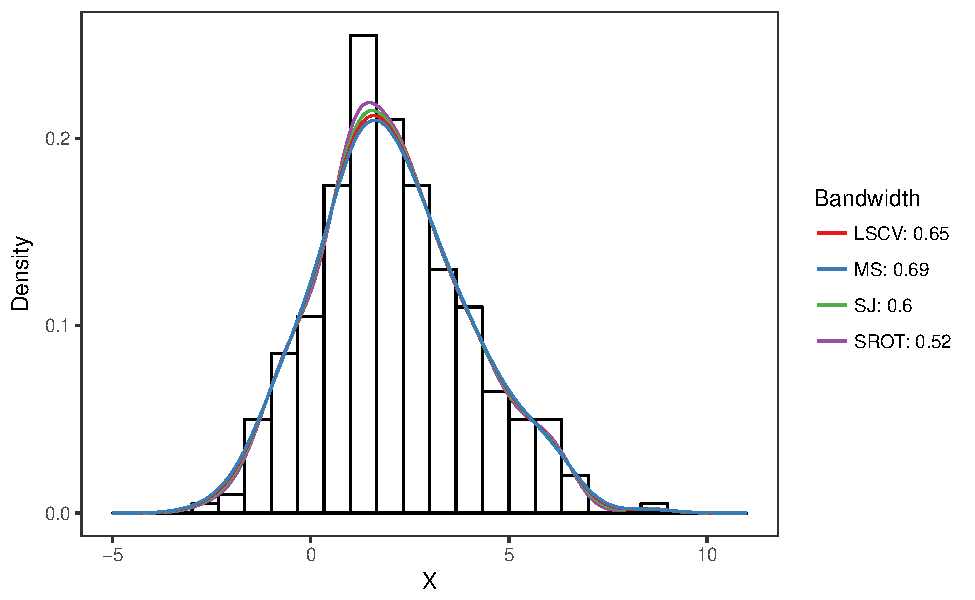
\includegraphics{FinalReport_files/figure-latex/unnamed-chunk-6-1} \end{center}

We begin by examining \(\widehat{f}_h(x)\) for a data vector sampled
solely from \(N(2, 2^2)\). In this case, we see that each bandwidth
selection does a fairly good job of estimating the density. \(h_{SROT}\)
relies on a normal approximation, so we would expect this bandwidth to
perform well on this vector. In fact, it is the most aggressive
bandwidth estimator, resulting in the smallest \(h\) value of the four.
A \emph{best bandwidth} is not apparent from these results.

\newpage

\subsection{Example 2: 50/50 Mixture of $N(0, 1)$ and $N(4, 2^2)$}

\begin{verbatim}
##           LS CV            T MS           SJ BW Silverman's ROT 
##           0.562           0.944           0.515           0.742
\end{verbatim}

\begin{center}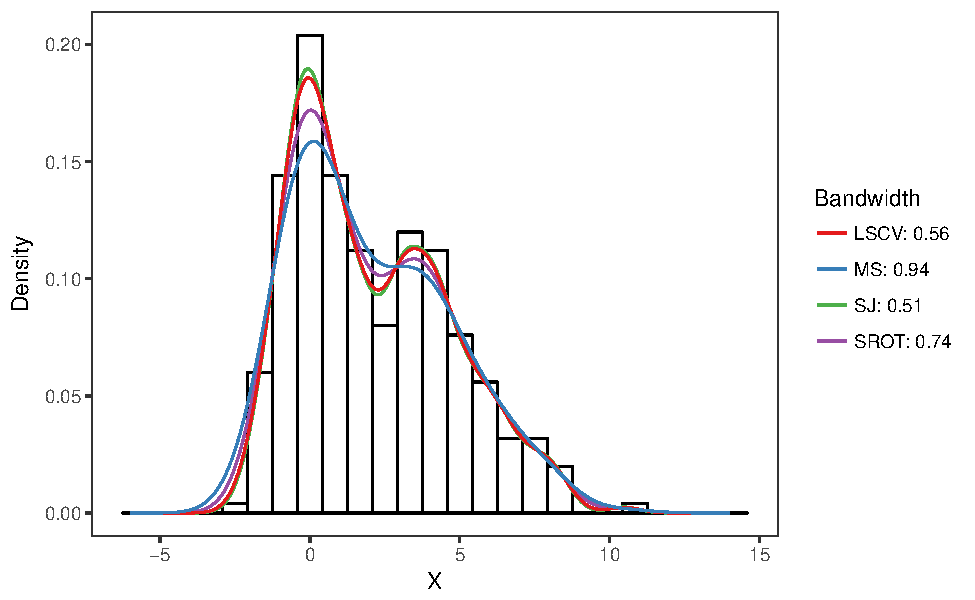
\includegraphics{FinalReport_files/figure-latex/unnamed-chunk-7-1} \end{center}

Moving on to a somewhat harder density to estimate, we simulate a 50/50
distribution coming from \(N(0,1)\) and \(N(2, 2^2)\). \(h_{SJ}\) and
\(h_{LSCV}\) both seem to capture the bimodality of the distribution
quite well. \(h_{SROT}\) smooths out some of the interesting features,
but the bimodality is still somewhat detectable. \(h_{MS}\) over-smooths
disastrously - without knowing the underlying structure of the data, it
would not be obvious that the data came from a bimodal distribution.

\newpage

\subsection{Example 3: Mixture of $\Gamma(\alpha = 1, \beta = 1/20)$, $\Gamma(\alpha = 4, \beta = 1/5)$, $\Gamma(\alpha = 20, \beta = 1)$}

A mixture of gamma distributions may seem like a ``toy'' example, but
the gamma distribution can be very helpful in modeling rainfall (e.g.
Husak, Michaelsen, and Funk (2007)).

\begin{verbatim}
##           LS CV            T MS           SJ BW Silverman's ROT 
##           1.382           4.514           2.241           2.374
\end{verbatim}

\begin{center}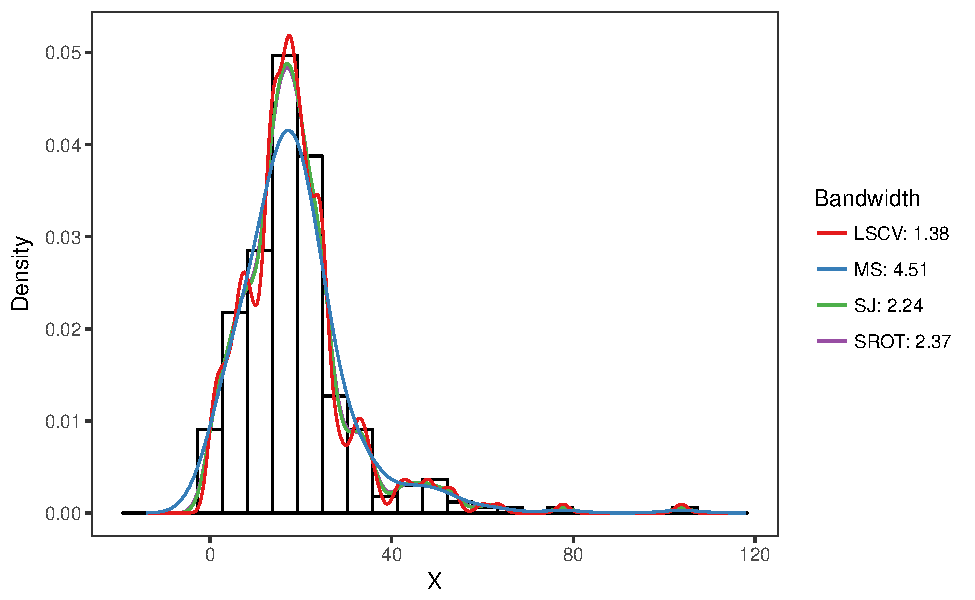
\includegraphics{FinalReport_files/figure-latex/unnamed-chunk-8-1} \end{center}

Here we see the excessive variation caused by using \(h_{LSCV}\). The
density estimate provided by \(h_{LSCV}\) is far too wiggly to be useful
for a data analyst. We also see that \(h_{MS}\) provides a much smoother
estimate than the those proposed by Silverman and Sheather and Jones, it
seems that it is too conservative. The best bandwidth would take a value
somewhere in the neighborhood of \(h_{SJ}\) and \(h_{SROT}\).

\newpage

\subsection{Example 4: Old Faithful Waiting Time}

\begin{verbatim}
##           LS CV            T MS           SJ BW Silverman's ROT 
##           2.190           5.081           2.560           3.998
\end{verbatim}

\begin{center}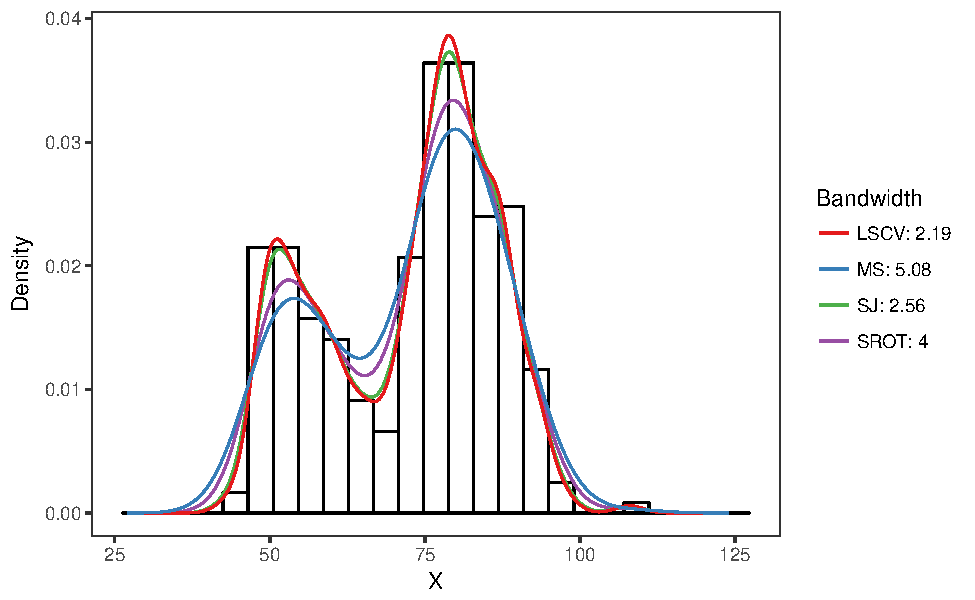
\includegraphics{FinalReport_files/figure-latex/unnamed-chunk-9-1} \end{center}

Using data from Azzalini and Bowman (1990), contained in the
\textbf{\texttt{MASS}} package (Venables and Ripley 2002), we calculate
the kernel density estimate for the waiting time for eruptions from
August 1 to August 15, 1985 at the Old Faithful geyser in Yellowstone
National Park, Wyoming.

Each bandwidth choice seems to capture the bimodality in the
distribution of waiting times with varying levels of success.
\(h_{LSCV}\) may be too aggressive, while \(h_{MS}\) does not reach far
enough up the left-side peak. \(h_{SJ}\) and \(h_{LSCV}\) seem grouped
together and \(h_{SROT}\) and \(h_{MS}\) seem grouped together as well.
Between \(h_{SJ}\) and \(h_{LSCV}\), we would want to choose the more
conservative bandwidth, which is \(h_{SJ}\). Conversely, between
\(h_{MS}\) and \(h_{SROT}\), we would want to choose the more aggressive
bandwidth, which is \(h_{SROT}\).

\section{Conclusion}\label{conclusion}

In this report we have presented four options for selecting a bandwidth
for univariate kernel density estimation. We have discussed bandwidths
that oversmooth (\(h_{MS}\)), and bandwidths that under-smooth
(\(h_{LSCV}\)). No universally optimal bandwidth selection has been
found, which makes selecting a bandwidth an iterative and subjective
process.

A safe option for a data analyst is to use at least two bandwidths when
analyzing the data. One bandwidth should have the tendency to
under-smooth (e.g. \(h_{SROT}\) or \(h_{MS}\)), and another bandwidth
should produce estimates that are more wiggly (e.g. \(h_{SJ}\),
\textbf{but not \(h_{LSCV}\)}). If visualizing is the goal (rather than
simulation), then including a histogram will provide even more clarity
when making density plots (note that making a histogram also requires
selecting a bandwidth, though).

In our \emph{Examples} section, we saw the devastating effects of
over-smoothing and under-smoothing. There is a large amount of
literature on univariate bandwidth selection, but a universally optimal
bandwidth has yet to be found. Selecting a bandwidth presents a
bias-variance tradeoff to the analyst, with a good bandwidth being
dependent on the analytical task. Sheather (2004, 596) suggests to
``produce a family of density estimates based on a number of values of
the bandwidth''. We agree with this suggestion, and believe it to be
sage advice for exploratory analysis.

\section{Question}\label{question}

Using the \texttt{density} function and the beer data
(\texttt{abv.complete}, which are the alcohol by volume measures for the
top 250 beers as rated by BeerAdvocate.com) provided below, compute and
plot a 95\% pointwise bootstrapped percentile interval. Additionally,
use the approximate variance function \(\tilde{V}\) given below and
found in Jann (2007, 2) to compute and plot a 95\% pointwise confidence
interval. Create two plots for each method using \texttt{bw.SJ} and
\texttt{bw.nrd0}.

\[\tilde{V}\left(\widehat{f_K}(x;h)\right) = \frac{1}{nh}R(K) \widehat{f_K}(x;h) - \frac{1}{n} \widehat{f_K}(x;h)^2\]

\begin{Shaded}
\begin{Highlighting}[]
\CommentTok{# data comes from the ABV of beer advocate's top 250 beers for 2016}
\CommentTok{# 2 beers have missing abv data}
\CommentTok{# quick R script to read in the .csv}
\KeywordTok{library}\NormalTok{(RCurl)}
\NormalTok{git_file <-}\StringTok{ }
\KeywordTok{getURL}\NormalTok{(}\StringTok{"https://raw.githubusercontent.com/bgstieber/Top250Beer/master/Top250Beers.csv"}\NormalTok{)}
\NormalTok{beer_data <-}\StringTok{ }\KeywordTok{read.csv}\NormalTok{(}\DataTypeTok{text =} \NormalTok{git_file, }\DataTypeTok{stringsAsFactors =} \OtherTok{FALSE}\NormalTok{)}
\NormalTok{abv.complete <-}\StringTok{ }\NormalTok{beer_data[!}\KeywordTok{is.na}\NormalTok{(beer_data$ABV), ]$ABV}
\end{Highlighting}
\end{Shaded}

\section{Solution}\label{solution}

\subsection{Bootstrap percentile
interval}\label{bootstrap-percentile-interval}

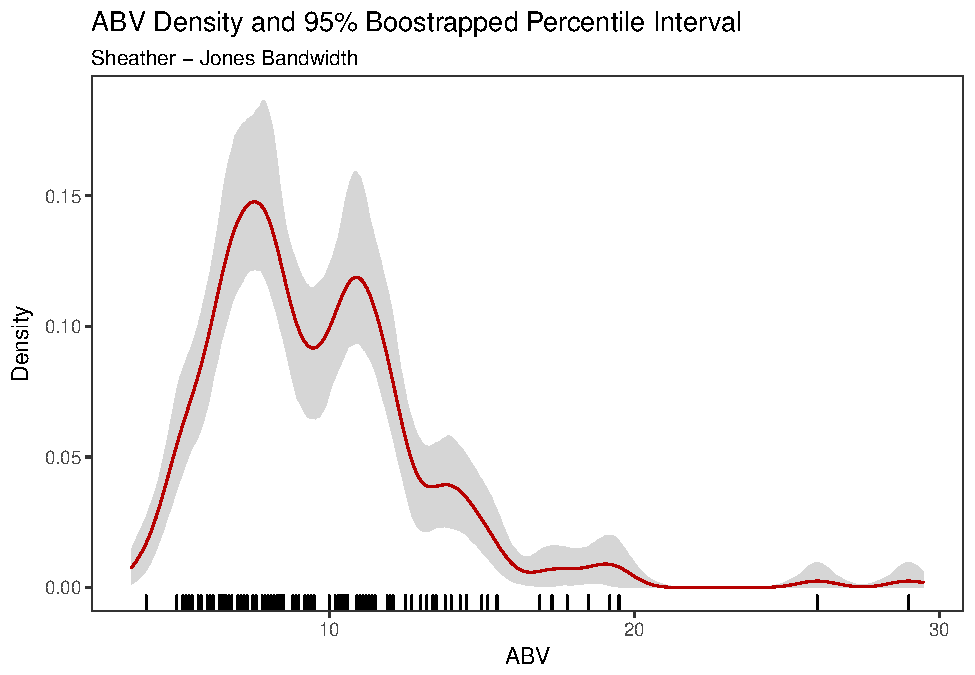
\includegraphics{FinalReport_files/figure-latex/unnamed-chunk-13-1.pdf}
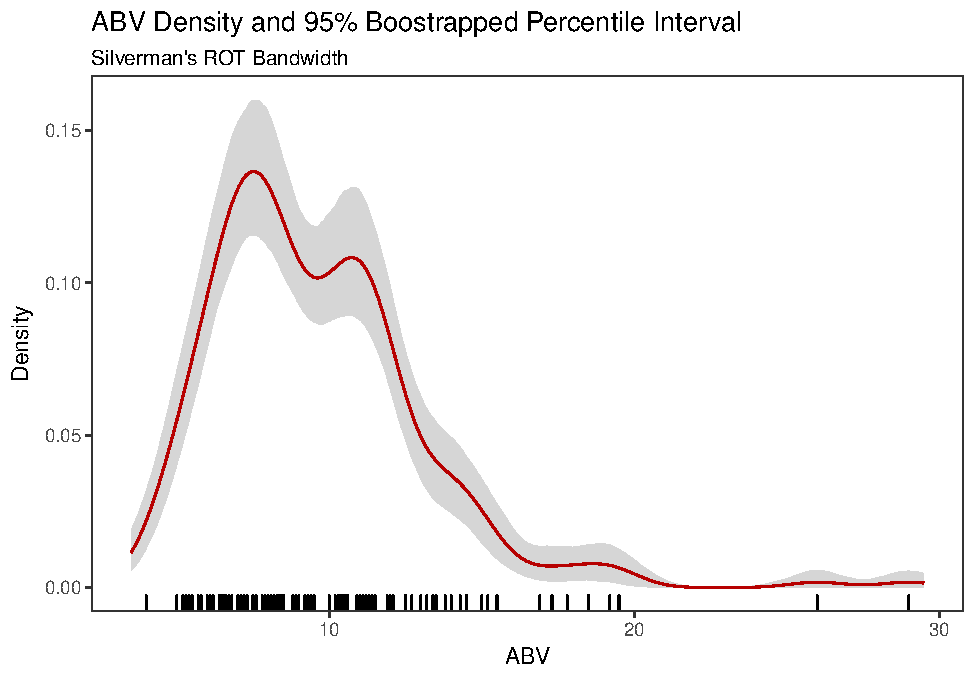
\includegraphics{FinalReport_files/figure-latex/unnamed-chunk-13-2.pdf}

\subsection{Approximate Confidence
Interval}\label{approximate-confidence-interval}

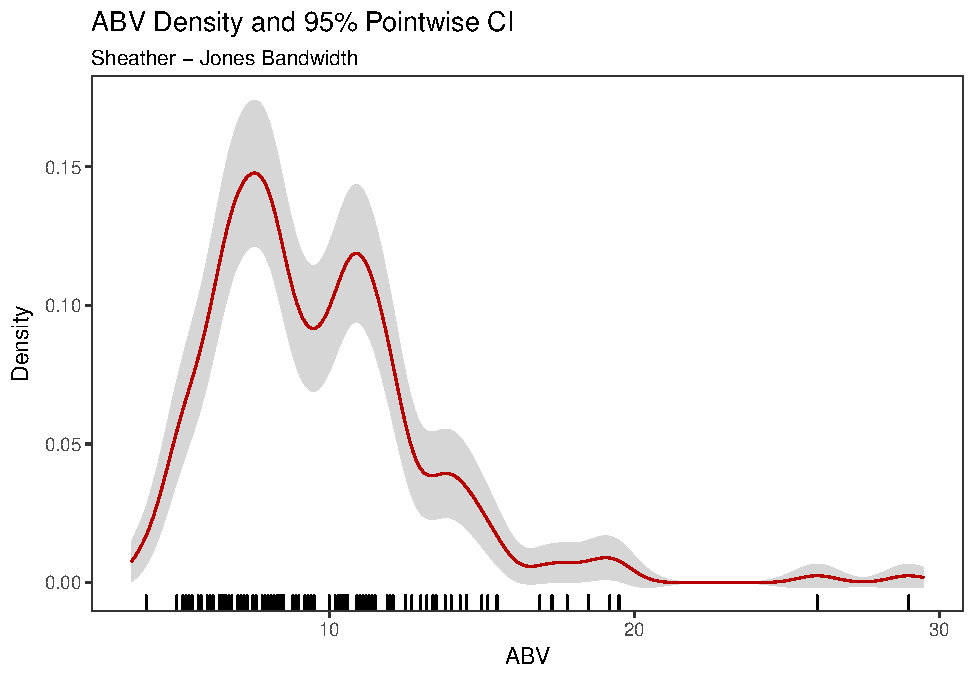
\includegraphics{FinalReport_files/figure-latex/unnamed-chunk-15-1.pdf}
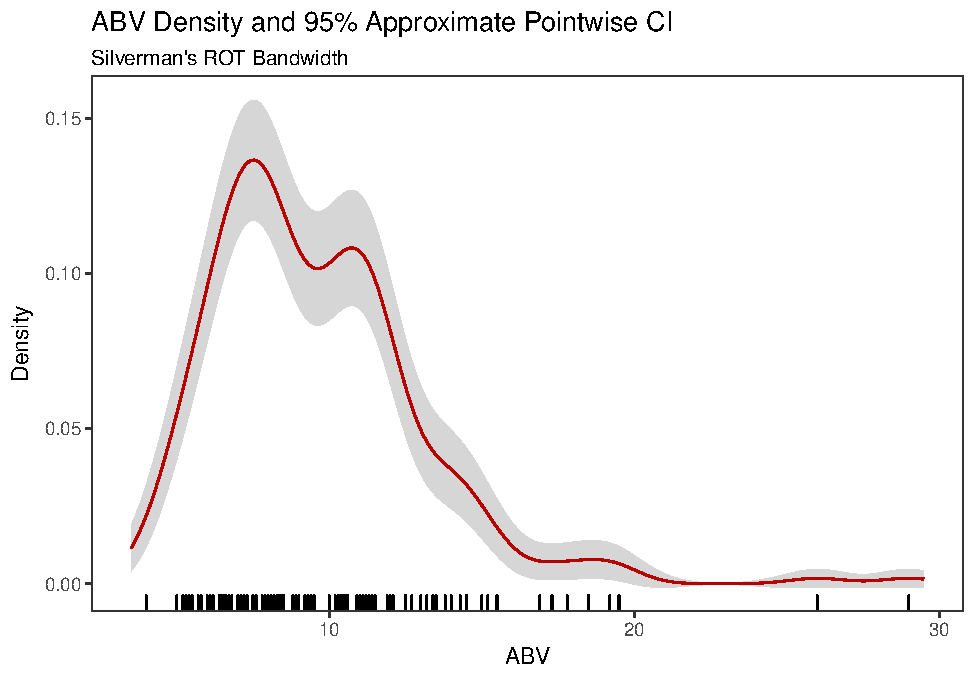
\includegraphics{FinalReport_files/figure-latex/unnamed-chunk-15-2.pdf}

\section{Appendix}\label{appendix}

\subsection{Shiny App Screenshots}\label{shiny-app-screenshots}

To visit the Shiny app,
\textbf{\href{http://www.statlab.wisc.edu/shiny/Bandwidths_For_UnivariateKDE/}{click
this link}}.

\begin{figure}[htbp]
\centering
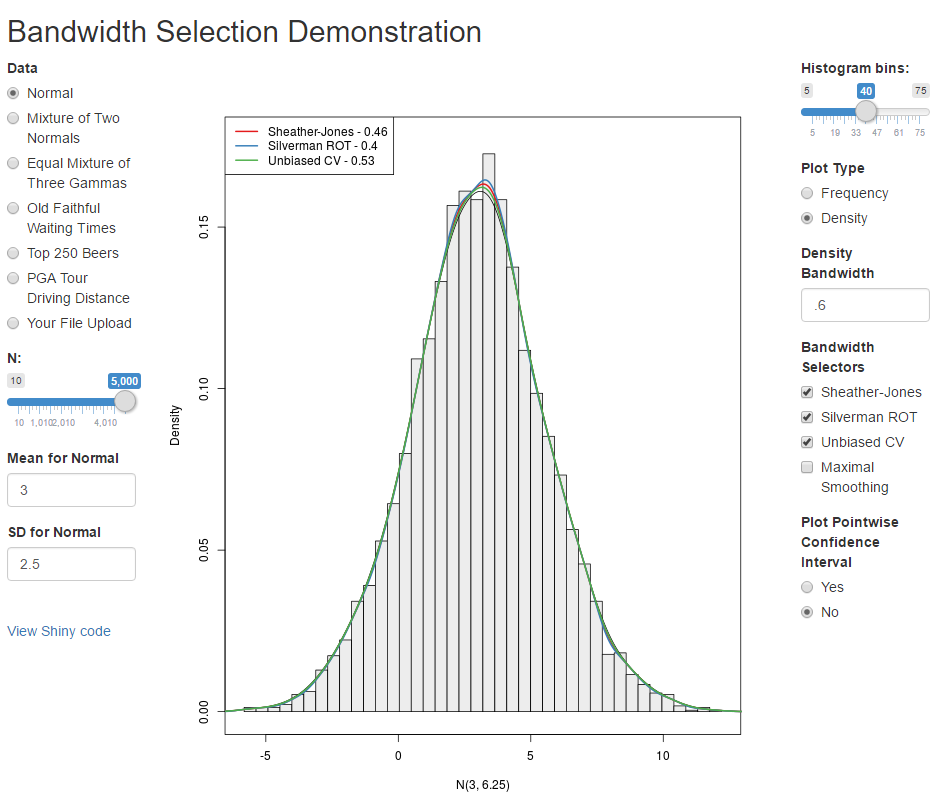
\includegraphics[width=0.6\textwidth]{ShinyScreenshot1.png}
\caption{Shiny app example of kernel density estimation using a normal distribution with the Sheather-Jones, Silverman, and CV bandwidths.}
\end{figure}

\begin{figure}
\centering
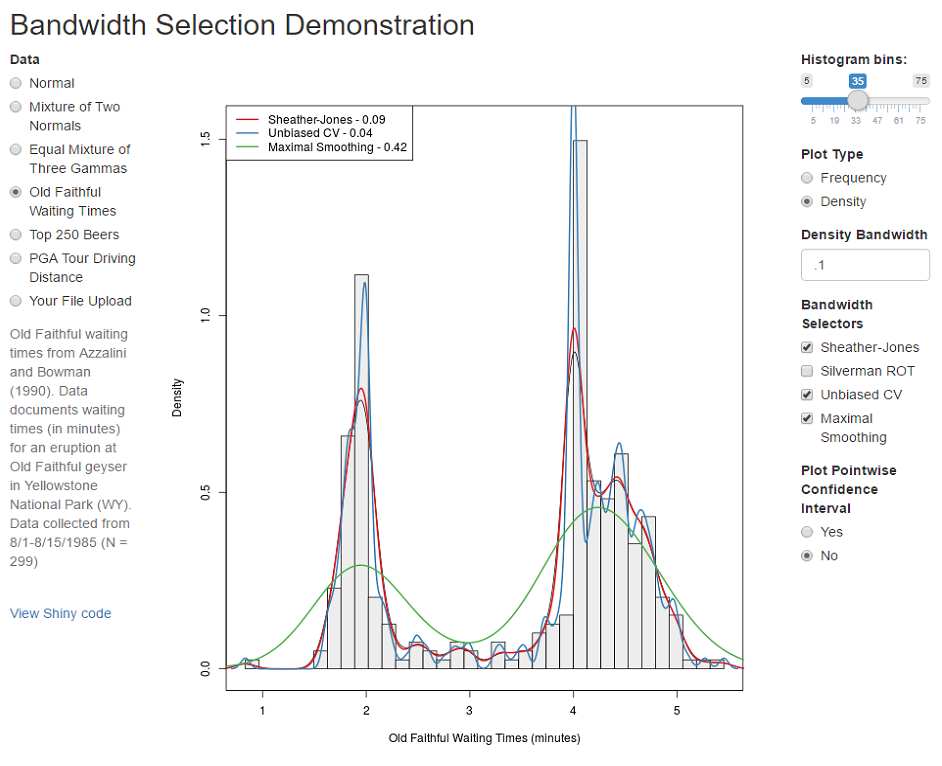
\includegraphics[width=0.6\textwidth]{ShinyScreenshot2.png}
\caption{Shiny app example of kernel density estimation using an equal mixture of gamma densities with the Sheather-Jones, CV, and Maximal Smoothing bandwidths.}
\end{figure}

\begin{figure}
\centering
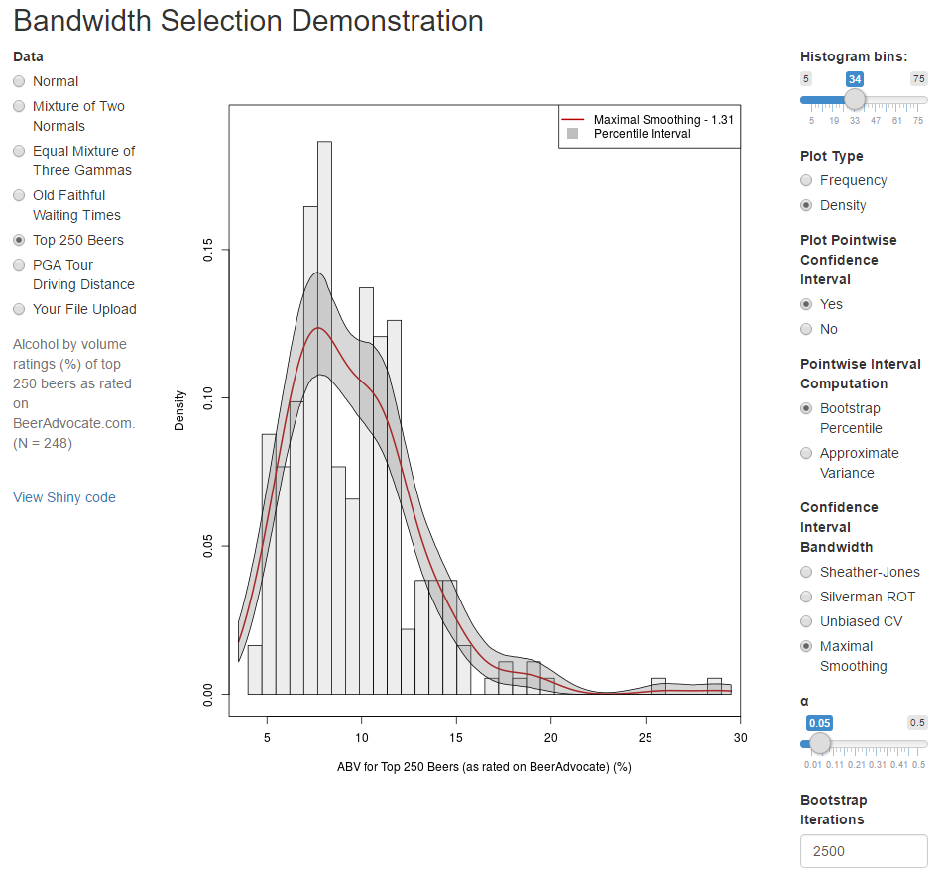
\includegraphics[width=0.6\textwidth]{ShinyScreenshot3.png}
\caption{Shiny app example of kernel density estimation with a bootstrapped pointwise interval on BeerAdvocate's ABV data. }
\end{figure}

\begin{figure}
\centering
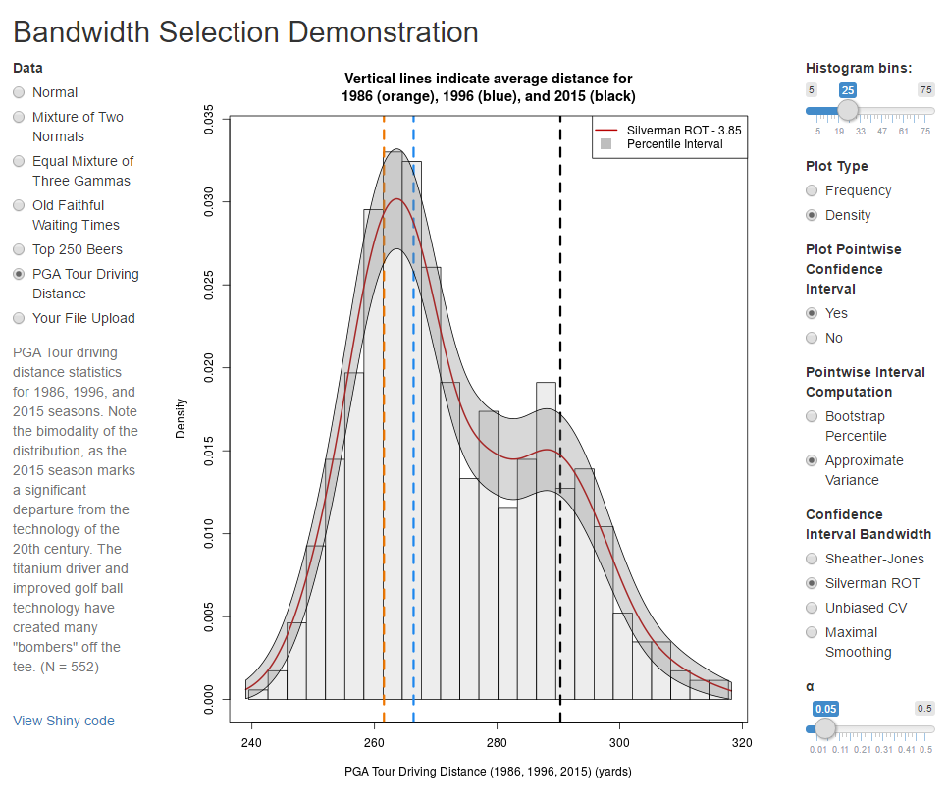
\includegraphics[width=0.6\textwidth]{ShinyScreenshot4.png}
\caption{Shiny app example of kernel density estimation with a pointwise confidence interval using the approximate variance calculation. The data we are visualizing are the average driving distances of PGA Tour players for 1986, 1996, 2006, and 2015.}
\end{figure}

\pagebreak

\subsection{Expression for Sheather-Jones
Bandwidth}\label{expression-for-sheather-jones-bandwidth}

As found in Givens and Hoeting (2013, 337), the Sheather-Jones bandwidth
can be found by solving the equation (using \(L = \phi\)):

\[
\left( \frac{R(K)}{n\sigma^4_K\hat{R}_{\hat{\alpha}(h)}(f'')} \right)^{1/5} - h = 0,
\]

where:

\[
\begin{aligned}
\hat{R}_{\hat{\alpha}(h)}(f'') &= \frac{1}{n(n-1)\alpha^5}\sum_{i = 1}^{n}\sum_{j=1}^{n}\phi^{(4)}\left(\frac{x_i - x_j}{\alpha}\right), \\
\hat{\alpha}(h) &= \left(\frac{6\sqrt{2}h^5\hat{R}_a(f'')}{\hat{R}_b(f''')}\right)^{1/7},\\
\hat{R}_a(f'') &= \frac{1}{n(n-1)a^5}\sum_{i = 1}^{n}\sum_{j=1}^{n}\phi^{(4)}\left(\frac{x_i - x_j}{a}\right), \\
\hat{R}_b(f'') &= \frac{1}{n(n-1)b^7}\sum_{i = 1}^{n}\sum_{j=1}^{n}\phi^{(6)}\left(\frac{x_i - x_j}{b}\right), \\
a &= \frac{0.920 IQR}{n^{1/7}} \\
b &= \frac{0.912 IQR}{n^{1/9}},
\end{aligned}
\]

where \(IQR\) is the interquartile range of the data, and \(\phi^{(i)}\)
is the ith derivative of the standard normal density function. To
determine the Sheather-Jones bandwidth in \texttt{R}, a user can write
\texttt{bw.SJ(x)}, which uses the \texttt{uniroot} function to perform
the root-finding.

\section*{References}\label{references}
\addcontentsline{toc}{section}{References}

\hypertarget{refs}{}
\hypertarget{ref-Bowman1990}{}
Azzalini, A, and A Bowman. 1990. ``A look at some data on the Old
Faithful geyser.'' \emph{Journal of the Royal Statistical Society} 39
(3): 357--65.
doi:\href{https://doi.org/10.2307/2347385}{10.2307/2347385}.

\hypertarget{ref-Givens2013}{}
Givens, Geof, and Jennifer Hoeting. 2013. \emph{Computational
Statistics}. 2nd ed. John Wiley \& Sons.

\hypertarget{ref-Husak2007}{}
Husak, Gregory J., Joel Michaelsen, and Chris Funk. 2007. ``Use of the
gamma distribution to represent monthly rainfall in Africa for drought
monitoring applications.'' \emph{International Journal of Climatology}
27.7 (June 2007): 935--44.
doi:\href{https://doi.org/10.1002/joc}{10.1002/joc}.

\hypertarget{ref-Jann2007}{}
Jann, Ben. 2007. ``Univariate kernel density estimation.''
\emph{Statistical Software Component}, no. 3.
\url{http://fmwww.bc.edu/RePEc/bocode/k/kdens.pdf}.

\hypertarget{ref-Jones1992}{}
Jones, M. C., J. S. Marron, and Simon J. Sheather. 1992. ``Progress in
data-based bandwidth selection for kernel density estimation.''
\emph{Computational Statistics} 11 (3): 337--81.

\hypertarget{ref-Jones1996}{}
---------. 1996. ``A brief survey of bandwidth belection for density
estimation.'' \emph{Journal of the American Statistical Association} 91
(433): 401--7.
doi:\href{https://doi.org/10.1080/01621459.1996.10476701}{10.1080/01621459.1996.10476701}.

\hypertarget{ref-Sheather2004}{}
Sheather, Simon J. 2004. ``Density estimation.'' \emph{Statistical
Science} 19 (4): 588--97.
doi:\href{https://doi.org/10.1214/088342304000000297}{10.1214/088342304000000297}.

\hypertarget{ref-Sheather1991}{}
Sheather, Simon J., and M. C. Jones. 1991. ``A reliable data-based
bandwidth selection method for kernel density estimation.''
\emph{Journal of the Royal Statistical Society} 53 (3): 683--90.

\hypertarget{ref-Silverman1986}{}
Silverman, Bernard W. 1986. \emph{Density Estimation for Statistics and
Data Analysis}. CRC press.

\hypertarget{ref-Terrell1990}{}
Terrell, George R. 1990. ``The maximal smoothing principle in density
estimation.'' \emph{Journal of the American Statistical Association} 85
(410): 470--77.
doi:\href{https://doi.org/10.2307/2289786}{10.2307/2289786}.

\hypertarget{ref-Venables}{}
Venables, W. N., and B. D. Ripley. 2002. \emph{Modern Applied Statistics
with S}. 4th ed. Springer. \url{http://www.stats.ox.ac.uk/pub/MASS4}.


\end{document}
